\part{Функциональные последовательности и ряды}
\section{Равномерно сходящиеся функциональные последовательности}

\begin{Def}
	Пусть $\{f_n(x)\}$ это последовательность функций, определённых в некоторой области $D \subset \bb{R}$, тогда говорят, что эта последовательность поточечно сходится к $F(x), x \in D$\\
	$\text{т.е. } \exists \lim\limits_{n \to +\infty} = F(x), (x \in D) \Leftrightarrow \forall x \in D \; \exists \lim\limits_{n \to +\infty} = F(x)\\
	\text{т.е. } \forall \varepsilon > 0 \; \exists N \in \bb{N}, N=N(\varepsilon, x) \; \forall n > N \; |f_n(x) - F(x)| < \varepsilon$
\end{Def}

\begin{Example}~\\
	\begin{figure}[h]
		\begin{minipage}[h]{0.55\linewidth}
			\center{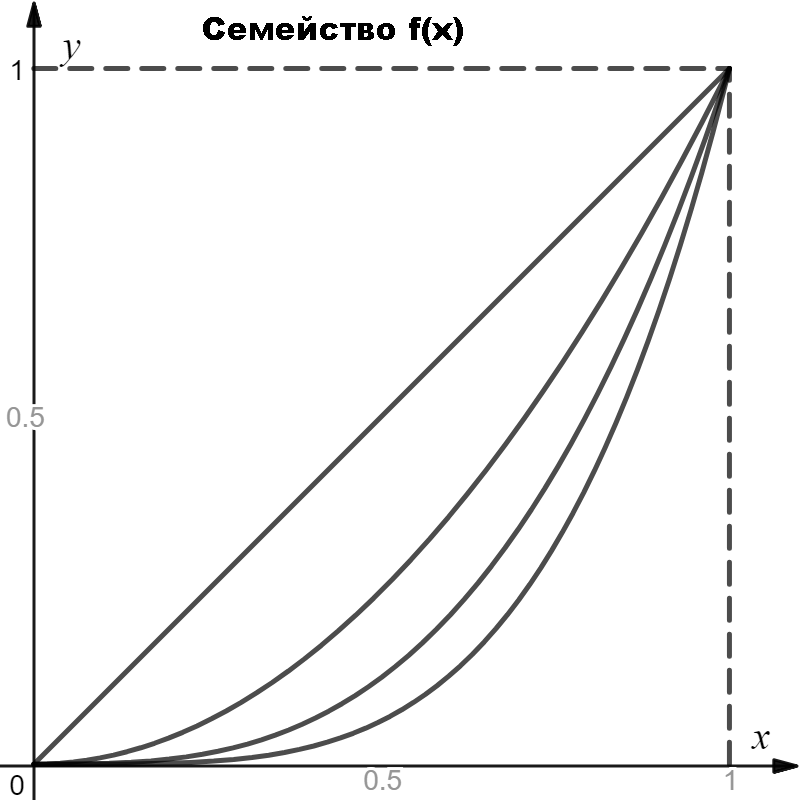
\includegraphics[width=0.75\linewidth]{pictures/4_1_1.png} \\ $\text{Семейство }f_n(x)$}
		\end{minipage}
		\hfill
		\begin{minipage}[h]{0.55\linewidth}
			\center{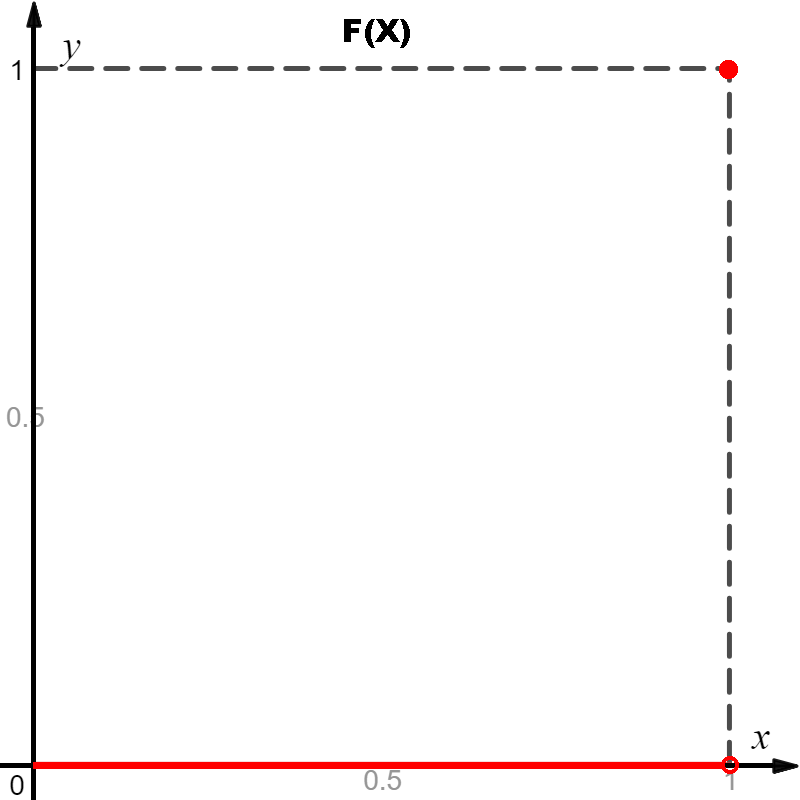
\includegraphics[width=0.75\linewidth]{pictures/4_1_2.png} \\ $F(x)$}
		\end{minipage}
	\end{figure}\\
	$f_n(x) = x^n, x \in [0;1]$\\
	$\lim\limits_{n \to +\infty}x^n = F(x) \Rightarrow F(x) = 
	\begin{cases}
	0, x \in [0;1)\\
	1, x=1
	\end{cases}$
\end{Example}

\begin{Def}
	Пусть $\{f_n(x)\}$ это последовательность функций, определённых в некоторой области $D \subset \bb{R}$, тогда говорят, что эта последовательность равномерно сходится к $F(x), x \in D \Leftrightarrow \\
	\Leftrightarrow \forall \varepsilon > 0 \; \exists N \in \bb{N}, N=N(\varepsilon, x) \; \forall n > N \; \forall x \in D \; |f_n(x) - F(x)| < \varepsilon$
	Отличие от поточечной сходимости получается только в том, что номер, с которого начинается пренебрежимо малое отставание от F не зависит от x\\
	Обозначают: $f_n(x) \rightrightarrows F(x) (n \to +\infty; x \in D)$
\end{Def}

\begin{Note}[Геометрический смысл равномерной сходимости]
	~\\
	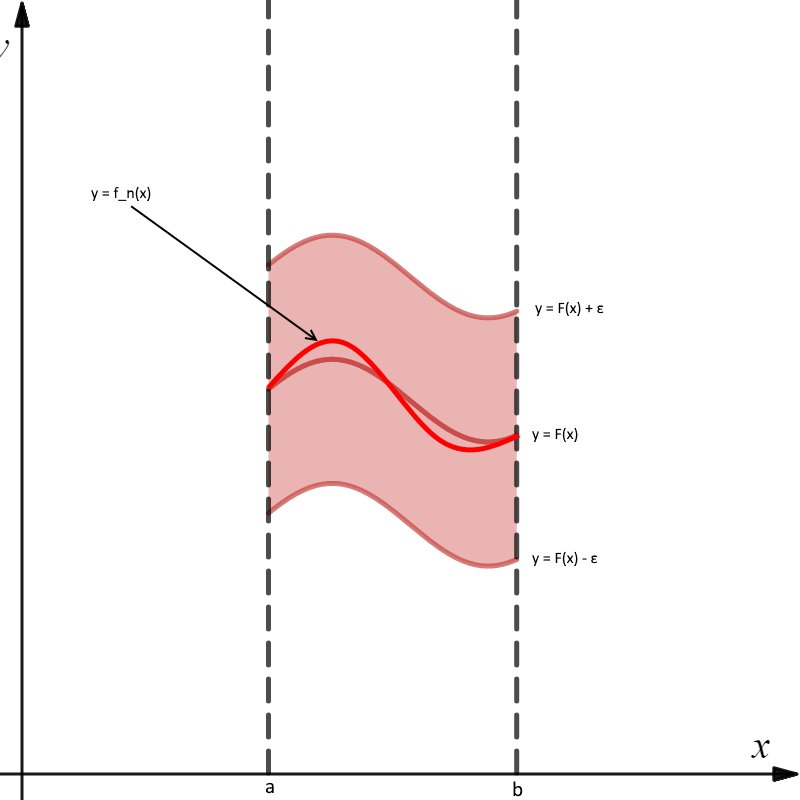
\includegraphics[width=0.5\linewidth]{pictures/4_1_3.png} $D = [a;b]$
\end{Note}

\begin{Note}
	~\\
	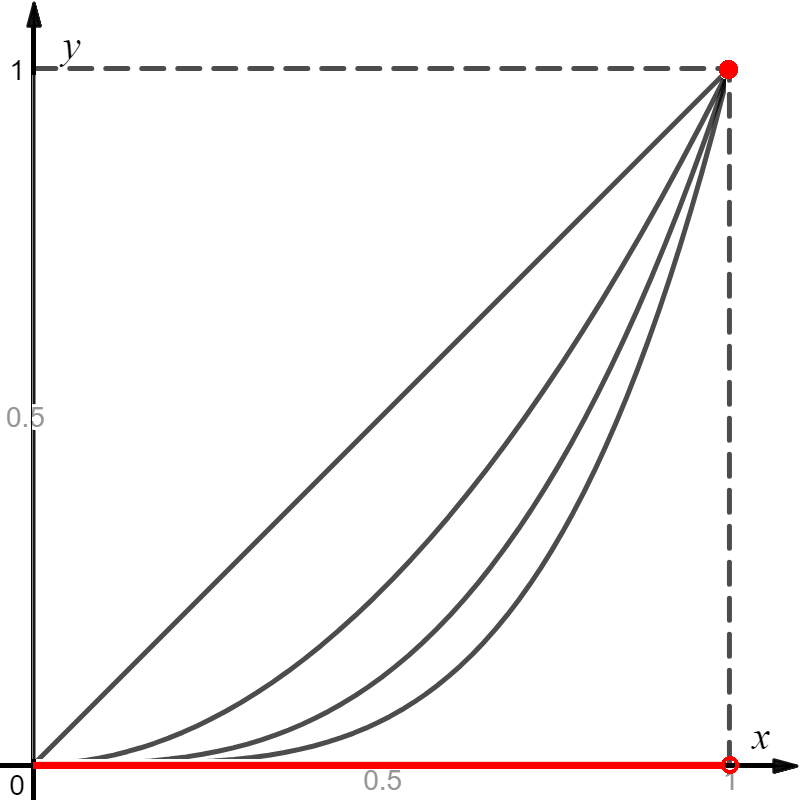
\includegraphics[width=0.5\linewidth]{pictures/4_1_4.png}\\
	$f_n(x) = x^n; x \in [0;1] \: \: f_n(x) \underset{n \to +\infty}{\rightarrow}F(x) \\
	f_n(x) \cancel{\rightrightarrows} F(x)$, где $F(x) = 
	\begin{cases}
	0, x \in [0;1)\\
	1, x = 1
	\end{cases} 0 < \varepsilon < \frac{1}{2}$
\end{Note}

\begin{Th}[Критерий Коши равномерной сходимости функциональных последовательностей]
	Пусть $\{f_n(x)\}$ - функциональная последовательность, где $x \in D$. Тогда $\{f_n(x)\}$ равномерно стремится к $F(x)$ при $n \to +\infty; x \in D \Leftrightarrow \\
	\Leftrightarrow \forall \varepsilon > 0 \; \exists N(\varepsilon) \in \bb{N} \; \forall n,m \geq N \; \forall x \in D \; |f_n(x)-f_m(x)| < \varepsilon$
\end{Th}

\begin{Proof}
	$\; \\ \Rightarrow \\$
	Пусть $f_n(x)$ равномерно сходится к $F(x)$ для $n \to +\infty, x \in D \Rightarrow \\$
	$\Rightarrow \forall n \geq N \; \forall x \in D \; |f_n(x) - F(x)| < \frac{\varepsilon}{2};\\$
	$\Rightarrow \forall m \geq N \; \forall x \in D \; |f_m(x) - F(x)| < \frac{\varepsilon}{2}\\
	|f_n(x) - f_m(x)| = |f_n(x) - F(x) + F(x) - f_m(x)| \leq |f_n(x) - F(x)| +\\
	+ |f_m(x) - F(x)| < \frac{\varepsilon}{2} + \frac{\varepsilon}{2} = \varepsilon \Rightarrow |f_n(x) - f_m(x)| < \varepsilon\\$
	$\; \\ \Leftarrow \\$
	$\forall \varepsilon \; \exists N(\varepsilon) \; \forall n,m \geq N \: |f_n(x) - f_m(x)| < \frac{\varepsilon}{2} \Rightarrow \\
	\text{Тогда} \; \forall x \in D \; f_m(x) \underset{n \to +\infty}{\rightarrow} F(x) $ (по критерию Коши для числовой последовательности)\\
	$\Rightarrow (m \to +\infty) \Rightarrow |f_n(x) - F(x)| \leq \frac{\varepsilon}{2} < \varepsilon \Rightarrow f_n(x) \rightrightarrows F(x) (n \to +\infty; x \in D)$
\end{Proof}

\begin{Th}[О непрерывности предела равномерно сходящихся функциональных последовательностей]
	Пусть $\forall n \geq 1 \text{ функции } f_n(x) \in C_{[a;b]}$.\\
	Тогда $f_n(x) \rightrightarrows F(x) (n \to +\infty, x \in [a;b]) \Rightarrow F(x) \in C_{[a;b]}$ 
\end{Th}

\begin{Proof}
	Надо доказать, что
	1. $\forall x_0 \in [a;b] \; \exists \lim\limits_{x \to x_0}F(x) = F(x_0) \text{и} 
	\begin{cases}
	\exists F(a+0) = F(a)\\
	\exists F(b-0) = F(b)
	\end{cases}\\$
	Пусть $x_0 \in [a;b], f_n(x) \in C_{[a;b]} \Rightarrow \text{[по теореме Кантора]} \Rightarrow \\
	\Rightarrow f_n(x) \text{равномерно непрерывна на} [a;b] \forall n in \bb{N},$\\
	т.е. $\forall \varepsilon > 0 \; \exists \delta > 0, \delta = \delta(\varepsilon, n) \; \forall x, x_0 \in [a;b] \; |x-x_0| < \delta \: |f_n(x)-f_n(x_0)| < \frac{\varepsilon}{3}$\\
	$f_n(x) \rightrightarrows F(x) (n \to +\infty; x \in D) \text{ для } \varepsilon > 0 \\
	\exists N \in \bb{N} \; \forall n \geq N \; \forall x, x_0 \in [a;b] |f_n(x) - F(x)| < \frac{\varepsilon}{3}, |f_n(x_0) - F(x_0)| < \frac{\varepsilon}{3}$\\
	Для $n = N: |f_N(x) - F(x)| < \frac{\varepsilon}{3}; |f_N(x_0) - F(x_0)| < \frac{\varepsilon}{3} \Rightarrow\\
	\Rightarrow |F(x) - F(x_0)| = |F(x) - f_N(x) + f_N(x) - F(x_0) - f_N(x_0) + f_N(x_0)| \leq \\
	\leq |f_N(x) - F(x)| + |f_N(x_0) - F(x_0)| + |f_N(x) - f_N(x_0)| < \frac{\varepsilon}{3} + \frac{\varepsilon}{3} + \frac{\varepsilon}{3} = \varepsilon$
	$\delta = \delta(\varepsilon, n)$, т.е. $\delta$ не зависит от $x$\\
	$\forall \varepsilon > 0 \; \exists N \in \bb{N} \; \exists \delta(\varepsilon, n) > 0 \; \forall x, x_0 \in [a;b] \; |x-x_0| < \delta \Rightarrow |F(x) - F(x_0)| < \varepsilon\\
	\Rightarrow F(x) \text{непрерывна на } [a;b]$
\end{Proof}

\begin{Note}
	$\lim\limits_{x \to x_0}(\lim\limits_{n \to +\infty}(f_n(x))) = \lim\limits_{n \to +\infty}(\lim\limits_{x \to x_0}(f_n(x))) \Leftrightarrow F(x) \in C_{[a;b]}, x,x_0 \in [a;b]$
\end{Note}

\begin{Th}[Об интегрировании равномерно сходящихся функциональных последовательностей]
	Пусть функции $f_n(x) \in C_[a;b]$ и $f_n(x) \rightrightarrows F(x), (n \to +\infty, x \in [a;b]) \Rightarrow\\
	\Rightarrow \exists \lim\limits_{n \to +\infty}\int\limits_{a}^{b}f_n(x)dx = \int\limits_{a}^{b}F(x)dx$
\end{Th}

\begin{Proof}
	$\; \\
	f_n(x) \rightrightarrows F(x) (n \to +\infty; x \in [a;b]) \Rightarrow\\
	\Rightarrow \forall \varepsilon > 0 \; \exists N(\varepsilon) \in \bb{N} \; \forall n \geq N \; \forall x \in [a;b] |f_n(x) - F(x)| < \frac{\varepsilon}{b - a}\\
	|\int\limits_{a}^{b}f_n(x)dx - \int\limits_{a}^{b}F(x)dx| = |\int\limits_{a}^{b}f_n(x)dx - F(x)dx| \leq \\
	\leq |\int\limits_{a}^{b}f_n(x)dx - F(x)dx| \leq \frac{\varepsilon}{b - a}(b-a) =  \varepsilon \Rightarrow\\
	\Rightarrow \forall \varepsilon > 0 \; \exists N(\varepsilon) \in \bb{N} \; \forall n \geq N \; \forall x \in [a;b] |\int\limits_{a}^{b}f_n(x)dx - \int\limits_{a}^{b}F(x)dx| \leq \varepsilon \Rightarrow\\
	\Rightarrow \exists \lim\limits_{n \to +\infty}\int\limits_{a}^{b}f_n(x)dx = \int\limits_{a}^{b}F(x)dx$
\end{Proof}

\begin{Note}
	$\lim\limits_{n \to +\infty}\int\limits_{a}^{b}f_n(x)dx = \int\limits_{a}^{b} \lim\limits_{n \to +\infty}f_n(x)dx$
\end{Note}

\begin{Note}
	Теорема 3 неверна в случае поточечной, а не равномерной, сходимости.\\
	\begin{figure}[h]
		\begin{minipage}[h]{0.3\linewidth}
			\center{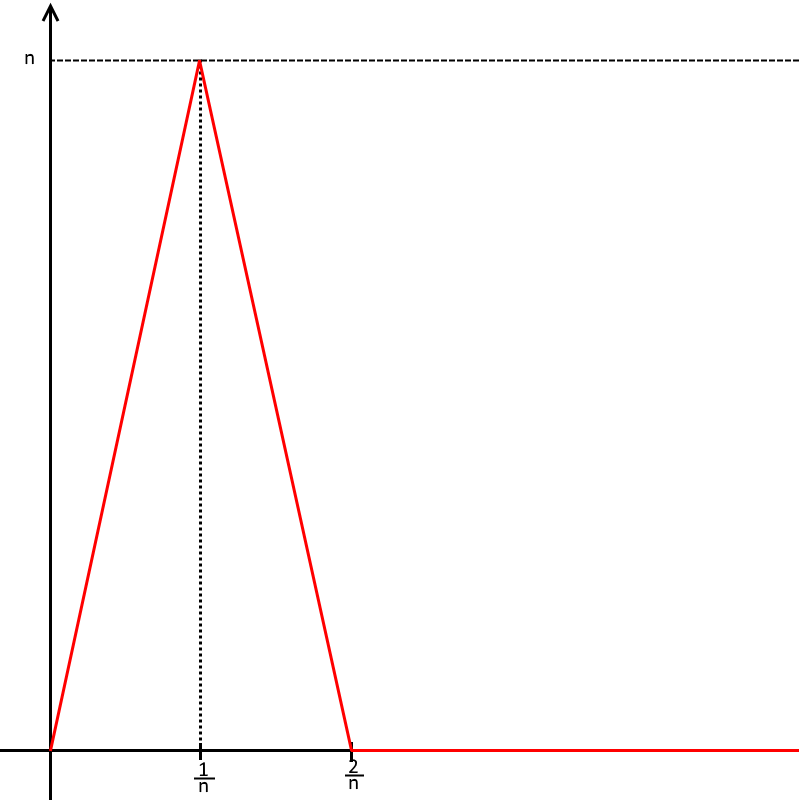
\includegraphics[width=0.9\linewidth]{pictures/4_1_5.png}}
		\end{minipage}
		\hfill
		\begin{minipage}[h]{0.7\linewidth}
			$f_n(x) \in C_{[0;1]}. f_n(x) \rightarrow 0 (n \to +\infty; x \in [0;1])\\
			\int\limits_{0}^{1}f_n(x) = \text{[как площадь треугольника]} = \frac{2}{n} \frac{n}{2} = 1 \rightarrow 1 (n \to +\infty)$\\
			Но при этом $\int\limits_{0}^{1}F(x) = 0 \rightarrow 0 (n \to +\infty) \Rightarrow\\
			\Rightarrow \lim\limits_{n \to +\infty}\int\limits_{a}^{b}f_n(x)dx \neq \int\limits_{a}^{b}F(x)dx$
		\end{minipage}
	\end{figure}\\
\end{Note}

\begin{Th}[О дифференциировании равномерно сходящихся функциональных рядов]
	Пусть $f_n(x) \in C_{[a;b]}^{1}, \text{т.е.} \exists f_n'(x) \in C_{[a;b]}$ и выполнены условия:\\
	\begin{enumerate}
		\item $f_n'(x) \rightrightarrows \varphi (x) (n \to +\infty; x \in [a;b])$
		\item $\exists x_0 \in [a;b] \; f_n(x_0) \rightarrow A (n \to +\infty)$
	\end{enumerate}
	Тогда:
	\begin{enumerate}
		\item $\exists F(x) \in C_{[a;b]}^{1} \; f_n(x) \rightrightarrows F(x) (n \to +\infty; x \in [a;b])$
		\item $F'(x) = \varphi'(x) (x \in [a;b])$
	\end{enumerate}
\end{Th}

\begin{Proof}
	$F(x) = A + \int\limits_{x_0}^{x}\varphi(t)dt$\\
	$\begin{cases}
	f_n'(x) \in C_{[a;b]}\\
	f_n'(x) \rightrightarrows \varphi(x)
	\end{cases} \Rightarrow \text{[по теореме 2]} \Rightarrow \varphi(t) \in C_{[a;b]} \Rightarrow\\
	\Rightarrow \varphi(t)$ интегрируема $\Rightarrow \text{[по теореме Барроу]} \Rightarrow \exists F'(x) = \varphi(x) (x \in [a;b])$\\
	$|f_n(x) - F(x)| = |\int\limits_{x_0}^{x}f_n'(t)dt + f_n(x_0) - A - \int\limits_{x_0}^{x}\varphi(t)dt| = \\
	= |\int\limits_{x_0}^{x}(f_n'(t) - \varphi(t))dt + f_n(x_0) - A| \leq |\int\limits_{x_0}^{x}|(f_n'(t) - \varphi(t))|dt| + |f_n(x_0) - A|$\\
	$\forall \varepsilon > 0 \; \exists N_1(\varepsilon) \in \bb{N} \; \forall n \geq N_1 \; \forall t \in [a;b] |f_n'(x) - \varphi(t)| < \frac{\varepsilon}{2(b-a)}$ т.к. $f_n(t)$ сходится к $\varphi(t)$\\
	Для $\varepsilon > 0 \exists N \geq N_1 \; \forall n \geq N \: |f_n(x_0) - A| < \frac{\varepsilon}{2}$\\
	Итого:\\
	$\forall \varepsilon > 0 \; \exists N(\varepsilon) \in \bb{N} \; \forall n \geq N \: |\int\limits_{x_0}^{x}|(f_n'(t) - \varphi(t))|dt| < \frac{\varepsilon}{2(b-a)}|\int\limits_{x_0}^{x}dt| = \\
	= \frac{\varepsilon |x-x_0|}{2(b-a)} \leq \frac{\varepsilon(b-a)}{2(b-a)} = \frac{\varepsilon}{2}$\\
	Прибавим к этому, что $|f_n(x_0) - A| < \frac{\varepsilon}{2}$ и получим:\\
	$|f_n(x) - F(x)| < \frac{\varepsilon}{2} + \frac{\varepsilon}{2} = \varepsilon$\\
	Итого:\\
	$\forall x \in [a;b] |f_n(x) - F(x)| < \varepsilon\\
	\forall \varepsilon > 0 \; \exists N(\varepsilon) \; \forall n \geq N \; \forall x \in [a;b] \: |f_n(x) - F(x)| < \varepsilon \Rightarrow f_n(x) \rightrightarrows F(x), (n \to +\infty, x \in [a;b])$ 1я часть доказана \textcolor{red}{Тут есть доказательство второй части, которое я пропустил или какой-то подвох?}
\end{Proof}
